\section{Systèmes d'administrations}\label{sec:rw:supervision:administration}
Les systèmes d'administrations informatiques permettent de gérer des parcs de ressources depuis le début des années 80 avec les premières mises en réseau d'équipements. Le principe étant de surveiller et surtout contrôler un système afin qu'il satisfasse les demandes des utilisateurs et les contraintes du propriétaire~\cite{Sloman:management}. Tant la supervision telle que nous l'entendons dans cette thèse se focalise sur le fait de traiter les données, ici le principe étant d'agir sur les équipements. Toutefois, les systèmes existant sont dotés d'une gestion de données, malheureusement trop ad-hoc la plupart du temps.

Cette section présente les systèmes d'administrations qui se conçoivent encore aujourd'hui pour exploiter des parcs de dispositifs à grande échelle. Ces systèmes sont spécifiés au travers de divers consortiums ou forums tels que le \textit{BroadBand Forum} (BBF) (portés par les opérateurs télécoms), le \textit{Forum Universal Plug'n'Play} (UPnP) (portés par l'électronique grand publique), ou encore \textit{Distributed Management Task Force} (DMTF), l'\textit{Institute of Electrical and Electronics Engineers} (IEEE) et l'\textit{Internet Engineering Task Force} (IETF), organisations ouvertes où participent entreprises, laboratoires et indépendants. Ces ententes permettent la spécification des standards autant au niveau des protocoles de communications que sur les modèles de données manipulés.

Tout d'abord, cette section présente la structure et la gestion des données issues des ressources. Ensuite, nous présenterons l'ensemble des possibilités de traitement. Et enfin, nous synthétiserons cette présentation grâce à la grille d'analyse.
\subsection{Architecture de gestion des données}
L'architecture de la gestion des données dans les systèmes classiques d'administration est principalement fondé sur des gestionnaires agents~\cite{CCITT:X700} (voir fig.~\ref{fig:rw:supervision:administration}). Cette architecture est celle utilisée de nos jours dans les protocoles d'administrations tels que TR-069~\cite{BBF:tr069}, UPnP Device Management~\cite{UPnP:MD}, mais aussi sur des protocoles plus anciens tels que SNMP~\cite{IETF:SNMP}. Le principe étant que sur les dispositifs devant être administrés est présent un module logiciel. Celui-ci comporte un agent capable de maintenir une petite base de données sous un format particulier représentant les données et état du système. Un gestionnaire est capable par la suite de transmettre les informations de l'agent à un système d'administration global qui agrégera l'ensemble des dispositifs.
\begin{figure}[ht]
    \centering
    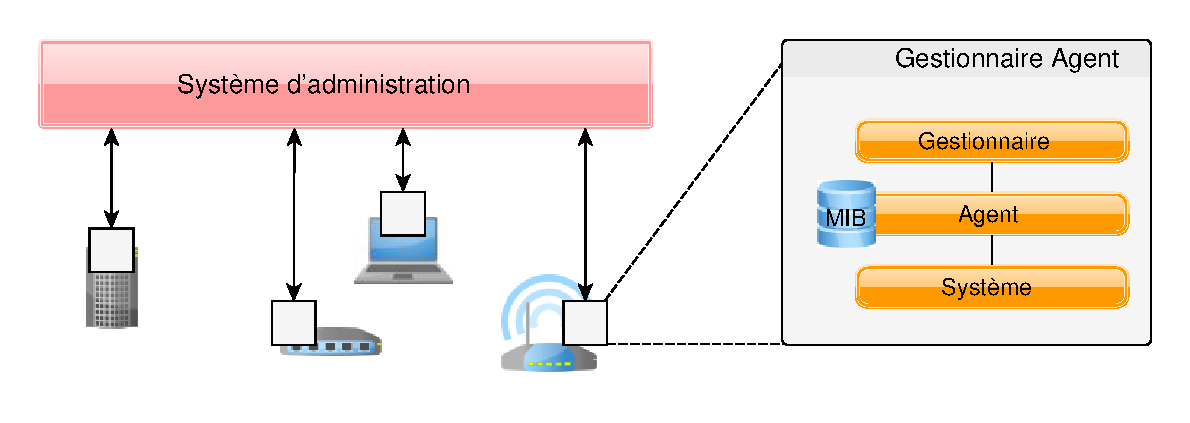
\includegraphics[width=.75\textwidth]{fig/rw-supervision-administration}
    \caption{Architecture d'un système classique d'administration}\label{fig:rw:supervision:administration}
\end{figure}

\subsubsection{Les données fournies les agents}
Il existe plusieurs structures abstraites de données dans le cadre des systèmes d'administrations. La structure la plus répandue reste en l'état la \textbf{structure hiérarchique}. La première apparition d'un tel modèle de donnée remonte à la spécification de SNMP qui prévoit le concept de \textit{Management Information Base} (MIB)~\cite{IETF:MIB}. Une \textit{MIB} est une base d'information où les données sont regroupées sous forme d'arbre. Chaque information possède à l'intérieur de ce arbre un chemin unique (l'\textit{object identifier}) décrit par une suite de chiffres séparés de points. Par exemple, \verb|1.3.6.1.2.1.2.2.1.2| est le chemin décrivant le nom d'une interface réseau sur un dispositif (par exemple \textit{eth0} sur un système Linux). Et le sous-arbre \verb|1.3.6.1.2| (MIB-II~\cite{IETF:MIB-II}) contient toutes les informations concernant les informations réseaux du dispositif.

Par la suite, l'idée des structures hiérarchiques a été reprise pour créer les protocoles d'administrations plus récents comme la structure du modèle des dispositifs de TR-069 (décrit dans le TR-106~\cite{BBF:tr106}) et dans le service de gestion de configuration (CMS) de UPnP-DM~\cite{UPnP:DMCMS}. Dans ces derniers, le modèle de donnée est décrit comme un système de fichier. Les \textit{instances} sont assimilables à des dossiers, et les \textit{feuilles} sont assimilables à des fichiers. Les nœuds ont ainsi un nom et un chemin unique vers la racine \enquote{/}. Tout comme leurs analogues, les \textit{instances} n'ont pas de valeurs associées alors que les \textit{feuilles} contiennent une donnée. Il existe plusieurs types d'\textit{instances} :
\begin{itemize}
    \item \textit{Unique} : Ce nœud peut contenir tout autre nœud. Il représente simplement un chemin intermédiaire un groupe de données.
    \item \textit{Multiple} : Ce nœud peut contenir plusieurs nœuds de type \textit{Instance}. Il permet de représenter une liste de nœuds similaires.
    \item \textit{Instance} : Il représente l'élement de la liste définie par l'instance multiple. Son nom sera toujours un entier pour l'identifier parmi les autres instances. Ces nœuds ont pour vocation à être créés ou supprimés en fonctionnement.
\end{itemize}
\begin{figure}[ht]
    \centering
    \includegraphics[width=.75\textwidth]{fig/rw-supervision-dmtree}
    \caption{Structure hiérarchique du modèle de données d'UPnP-DM}\label{fig:rw:supervision:dmtree}
\end{figure}


Un exemple de modèle de données de ce type de structure est présenté en figure~\ref{fig:rw:supervision:dmtree}. Désormais, une donnée est définie de manière unique, tout comme dans la MIB, grâce à son chemin complet. Dans le vocabulaire du domaine de l'administration, cette donnée est appelé \textit{paramètre}. Le \textit{chemin} d'un paramètre est la concaténation des noms des nœuds qui le sépare de la racine, avec pour séparateur \enquote{/} dans UPnP ou \enquote{.} dans TR-069. Voici quelques exemples de paramètres :
\begin{itemize}
\item \verb|/UPnP/DM/DeviceInfo/PhysicalDevice/HardwareVersion| permet de connaître la version du matériel du dispositif administré. 
\item \verb|/UPnP/DM/Configuration/Network/IPInterface/3/SystemName| est le nom d'une des interfaces réseaux (tout comme \verb|1.3.6.1.2.1.2.2.1.2| dans la MIB). En remplaçant \verb|/3/| par \verb|/5/|, cela concernera une autre interface réseau.
\end{itemize}

L'implémentation de l'agent permettra par la suite de pouvoir créer et remplir cette base d'information.
 
\begin{figure}[ht]
    \centering
    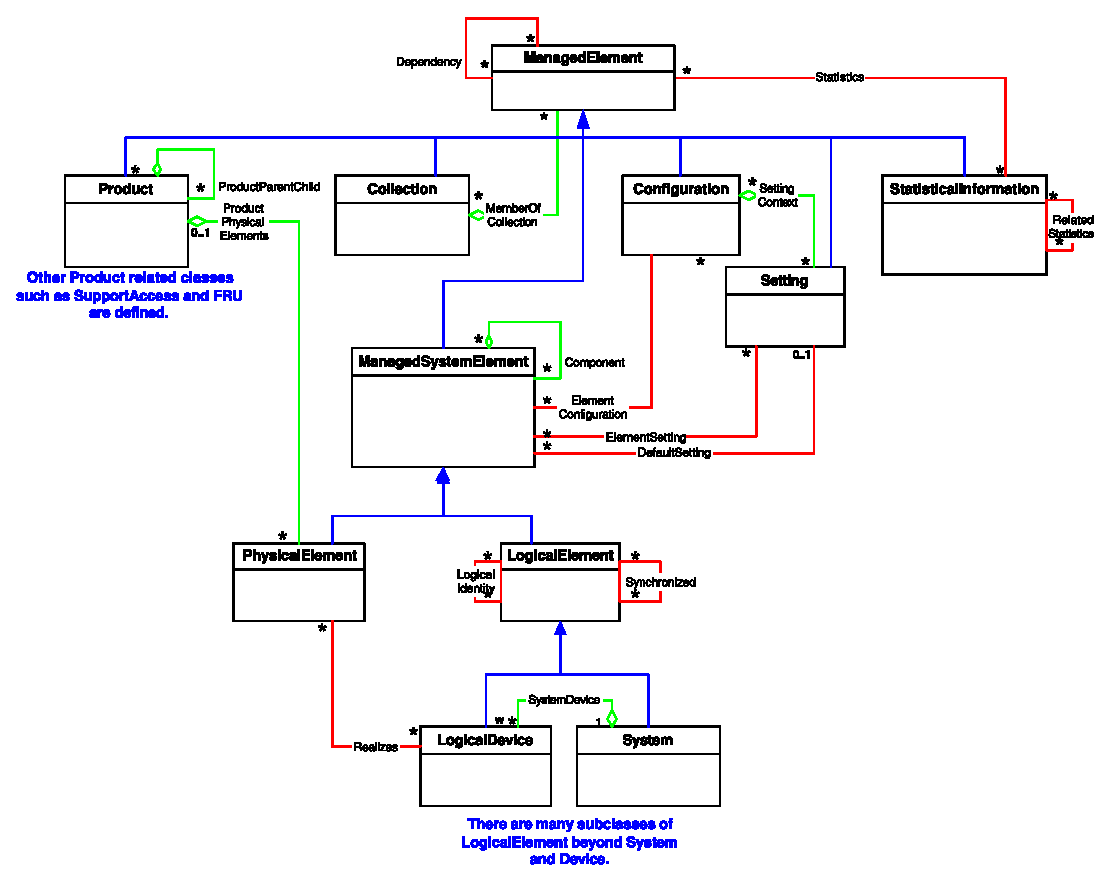
\includegraphics[width=.75\textwidth]{fig/rw-supervision-cimcore}
    \caption{Modèle de classe de la partie \textit{Core} de \textit{CIM}}\label{fig:rw:supervision:cimcore}
\end{figure}
Toutefois, tous les modèles ne sont pas tous orientés sur la hiérarchie. Il existe notamment l'approche objet adoptée dans les protocoles issues de la DMTF. En effet, dans les protocoles tels que WBEM ou WS-MAN~\cite{DMTF:WS-MAN} proposés par le DMTF, la fondation du modèle de données est décrite par un diagramme de classe UML comme présenté en figure~\ref{fig:rw:supervision:cimcore}. Nous pouvons remarquer la présence des différents concepts des structures précédentes avec le concept de \textit{Settings}, de \textit{ManagedElement}, et de \textit{Collection}. Plusieurs extensions standardisées existent pour modéliser les différents aspects des systèmes : Base de données, Dispositifs, Réseau, Sécurité, Utilisateur, Applications\dots{} Ainsi, le modèle des données sera un modèle d'objet respectant l'ensemble des spécifications et des extensions. L'inconvénient majeur d'un tel choix de méta-modèle restant la complexité de CIM qui se trouve souvent réduite pour être applicable en pratique.

Le système se compose ainsi de multiples agents qui seront une représentation de chacun des objets. Les objets du systèmes sont ainsi exposés à un service de gestion pour en fournir plusieurs propriétés. Nous pouvons noter que ce principe reste le même pour l'administration de modules Java dans le protocole JMX~\cite{Sun:JMX} où des objets particuliers (les \textit{MBean}) sont exposés et peuvent être consultés ou manipulés via ce protocole.

\subsubsection{Dynamisme des données}


\subsubsection{Le gestionnaire global}
Dans l'architecture présentée en figure~\ref{fig:rw:supervision:administration}, de multiples agents fournissent différentes informations selon les modèles présentés dans la section précédente. Le système d'administration se connecte aux différents agents afin de les gérer. Il sert à la fois d'interface à l'utilisateur que d'infrastructure de collecte et de d'analyse. En effet, l'intégration des données ainsi que la vue globale du système se constituera à l'intérieur de celui-ci.

Il est important de noter que ce système peut ne pas être centralisé pour mieux amortir la charge en la présence de grande quantités d'agents à administrer. Toutefois, il est important de voir que pour de l'administration de dispositifs des architectures centralisés peuvent suffir. Par exemple, pour l'administration de ses dispositifs, \textit{France Telecom} utilise un \textit{ACS} (serveur d'administration en TR-069) centralisé. En effet, la fréquence d'émission des données en fonctionnement normal se compte en jour pour chaque dispositif. Pour les 10 millions d'équipement à gérer, une capacité de 500 réceptions par seconde côté serveur est suffisante. Cette capacité est atteinte sur des \textit{ACS} récent tels que \textit{EDGE} de \textit{Motorola} sur des serveurs de capacité standardes.

Toutefois, plus l'usage le requiert, plus ce type d'architecture ne pourra supporter la charge des informations remontées. Plusieurs systèmes d'administrations supportent des structures hiérarchiques pour la gestion à plus grande échelle~\cite{Kessis:management}. La hiérarchie peut se découper par lieu géographique, ou par domaine d'activité. Dans le cadre des gestions par objets, le découpage par domaine permettra de répartir l'ensemble des agents par unité de traitement.

La section suivante présente les capacités de traitements de ce type de systèmes.

\subsection{Possibles traitements de données}
\subsubsection{L'hétérogénéité par la standardisation}
\subsubsection{Intégration de sources}
\subsubsection{Statistiques}
\subsubsection{Extension du modèle}
\subsection{Synthèse}

\begin{table}[ht]
\criteretabDonnee
    {Principalement structure \textbf{hiérarchique} sous forme de système de fichier. Quelques systèmes d'administration utilisent des modèles objets avec CIM, mais reste difficile à maîtriser.}
    {Une donnée est identifié par son chemin complet. La sémantique est décrite par ce chemin. Pas de contraintes ou inférences exprimées.}
    {Le dynamisme est géré par le mode d'accès. Certains nœuds peuvent être notifiables. D'autres ne sont actualisés que par consultation.}
\criteretabTraitement
    {Instantané et continu sur certaines données. Pas d'hybride possible vu que les procédés sont très séparés.}
    {Standardisation des modèles. Toutes les entités sont structurés dans le même formalisme. Intégration par union des résultats.}
    {Appel de méthodes standardes pour récupérer un sous-arbre du modèle. Code impératif (scripting) pour manipuler les données au niveau du gestionnaire.}
    {Projection simple sur les appels. Certains nœuds particuliers permettent de calculer des statistiques.}
\criteretabAdaptabilite
    {Pas d'adaptation car les dispositifs doivent implémenter des standards.}
    {Pas de perspectives métiers en dehors de la sélection sur les branches du modèle.}
    {Nœuds particuliers pour le calcul. Fonctions métiers intégrées dans le gestionnaire.}
    {Très efficace et utilisé pour gérer des parcs de millions de dispositifs.}
\end{table}